% Options for packages loaded elsewhere
\PassOptionsToPackage{unicode}{hyperref}
\PassOptionsToPackage{hyphens}{url}
\PassOptionsToPackage{dvipsnames,svgnames,x11names}{xcolor}
%
\documentclass[
  letterpaper,
  DIV=11,
  numbers=noendperiod]{scrartcl}

\usepackage{amsmath,amssymb}
\usepackage{iftex}
\ifPDFTeX
  \usepackage[T1]{fontenc}
  \usepackage[utf8]{inputenc}
  \usepackage{textcomp} % provide euro and other symbols
\else % if luatex or xetex
  \usepackage{unicode-math}
  \defaultfontfeatures{Scale=MatchLowercase}
  \defaultfontfeatures[\rmfamily]{Ligatures=TeX,Scale=1}
\fi
\usepackage{lmodern}
\ifPDFTeX\else  
    % xetex/luatex font selection
\fi
% Use upquote if available, for straight quotes in verbatim environments
\IfFileExists{upquote.sty}{\usepackage{upquote}}{}
\IfFileExists{microtype.sty}{% use microtype if available
  \usepackage[]{microtype}
  \UseMicrotypeSet[protrusion]{basicmath} % disable protrusion for tt fonts
}{}
\makeatletter
\@ifundefined{KOMAClassName}{% if non-KOMA class
  \IfFileExists{parskip.sty}{%
    \usepackage{parskip}
  }{% else
    \setlength{\parindent}{0pt}
    \setlength{\parskip}{6pt plus 2pt minus 1pt}}
}{% if KOMA class
  \KOMAoptions{parskip=half}}
\makeatother
\usepackage{xcolor}
\setlength{\emergencystretch}{3em} % prevent overfull lines
\setcounter{secnumdepth}{5}
% Make \paragraph and \subparagraph free-standing
\ifx\paragraph\undefined\else
  \let\oldparagraph\paragraph
  \renewcommand{\paragraph}[1]{\oldparagraph{#1}\mbox{}}
\fi
\ifx\subparagraph\undefined\else
  \let\oldsubparagraph\subparagraph
  \renewcommand{\subparagraph}[1]{\oldsubparagraph{#1}\mbox{}}
\fi


\providecommand{\tightlist}{%
  \setlength{\itemsep}{0pt}\setlength{\parskip}{0pt}}\usepackage{longtable,booktabs,array}
\usepackage{calc} % for calculating minipage widths
% Correct order of tables after \paragraph or \subparagraph
\usepackage{etoolbox}
\makeatletter
\patchcmd\longtable{\par}{\if@noskipsec\mbox{}\fi\par}{}{}
\makeatother
% Allow footnotes in longtable head/foot
\IfFileExists{footnotehyper.sty}{\usepackage{footnotehyper}}{\usepackage{footnote}}
\makesavenoteenv{longtable}
\usepackage{graphicx}
\makeatletter
\def\maxwidth{\ifdim\Gin@nat@width>\linewidth\linewidth\else\Gin@nat@width\fi}
\def\maxheight{\ifdim\Gin@nat@height>\textheight\textheight\else\Gin@nat@height\fi}
\makeatother
% Scale images if necessary, so that they will not overflow the page
% margins by default, and it is still possible to overwrite the defaults
% using explicit options in \includegraphics[width, height, ...]{}
\setkeys{Gin}{width=\maxwidth,height=\maxheight,keepaspectratio}
% Set default figure placement to htbp
\makeatletter
\def\fps@figure{htbp}
\makeatother
% definitions for citeproc citations
\NewDocumentCommand\citeproctext{}{}
\NewDocumentCommand\citeproc{mm}{%
  \begingroup\def\citeproctext{#2}\cite{#1}\endgroup}
\makeatletter
 % allow citations to break across lines
 \let\@cite@ofmt\@firstofone
 % avoid brackets around text for \cite:
 \def\@biblabel#1{}
 \def\@cite#1#2{{#1\if@tempswa , #2\fi}}
\makeatother
\newlength{\cslhangindent}
\setlength{\cslhangindent}{1.5em}
\newlength{\csllabelwidth}
\setlength{\csllabelwidth}{3em}
\newenvironment{CSLReferences}[2] % #1 hanging-indent, #2 entry-spacing
 {\begin{list}{}{%
  \setlength{\itemindent}{0pt}
  \setlength{\leftmargin}{0pt}
  \setlength{\parsep}{0pt}
  % turn on hanging indent if param 1 is 1
  \ifodd #1
   \setlength{\leftmargin}{\cslhangindent}
   \setlength{\itemindent}{-1\cslhangindent}
  \fi
  % set entry spacing
  \setlength{\itemsep}{#2\baselineskip}}}
 {\end{list}}
\usepackage{calc}
\newcommand{\CSLBlock}[1]{\hfill\break\parbox[t]{\linewidth}{\strut\ignorespaces#1\strut}}
\newcommand{\CSLLeftMargin}[1]{\parbox[t]{\csllabelwidth}{\strut#1\strut}}
\newcommand{\CSLRightInline}[1]{\parbox[t]{\linewidth - \csllabelwidth}{\strut#1\strut}}
\newcommand{\CSLIndent}[1]{\hspace{\cslhangindent}#1}

\KOMAoption{captions}{tableheading}
\makeatletter
\@ifpackageloaded{bookmark}{}{\usepackage{bookmark}}
\makeatother
\makeatletter
\@ifpackageloaded{caption}{}{\usepackage{caption}}
\AtBeginDocument{%
\ifdefined\contentsname
  \renewcommand*\contentsname{Table of contents}
\else
  \newcommand\contentsname{Table of contents}
\fi
\ifdefined\listfigurename
  \renewcommand*\listfigurename{List of Figures}
\else
  \newcommand\listfigurename{List of Figures}
\fi
\ifdefined\listtablename
  \renewcommand*\listtablename{List of Tables}
\else
  \newcommand\listtablename{List of Tables}
\fi
\ifdefined\figurename
  \renewcommand*\figurename{Figure}
\else
  \newcommand\figurename{Figure}
\fi
\ifdefined\tablename
  \renewcommand*\tablename{Table}
\else
  \newcommand\tablename{Table}
\fi
}
\@ifpackageloaded{float}{}{\usepackage{float}}
\floatstyle{ruled}
\@ifundefined{c@chapter}{\newfloat{codelisting}{h}{lop}}{\newfloat{codelisting}{h}{lop}[chapter]}
\floatname{codelisting}{Listing}
\newcommand*\listoflistings{\listof{codelisting}{List of Listings}}
\makeatother
\makeatletter
\makeatother
\makeatletter
\@ifpackageloaded{caption}{}{\usepackage{caption}}
\@ifpackageloaded{subcaption}{}{\usepackage{subcaption}}
\makeatother
\ifLuaTeX
  \usepackage{selnolig}  % disable illegal ligatures
\fi
\usepackage{bookmark}

\IfFileExists{xurl.sty}{\usepackage{xurl}}{} % add URL line breaks if available
\urlstyle{same} % disable monospaced font for URLs
\hypersetup{
  pdftitle={Inferência Estatística - um curso de graduação},
  pdfauthor={James D Santos},
  colorlinks=true,
  linkcolor={blue},
  filecolor={Maroon},
  citecolor={Blue},
  urlcolor={Blue},
  pdfcreator={LaTeX via pandoc}}

\title{Inferência Estatística - um curso de graduação}
\author{James D Santos}
\date{2025-12-08}

\begin{document}
\maketitle

\renewcommand*\contentsname{Table of contents}
{
\hypersetup{linkcolor=}
\setcounter{tocdepth}{2}
\tableofcontents
}
\bookmarksetup{startatroot}

\chapter*{Preface}\label{preface}
\addcontentsline{toc}{chapter}{Preface}

\markboth{Preface}{Preface}

Estas são as notas de aula do curso de Inferência Estatística,
ministradas durante o segundo semestre de 2024 e voltada para alunos de
graduação em estatística.

\bookmarksetup{startatroot}

\chapter{Summary}\label{summary}

Ementa: Conceitos básicos sobre amostras aleatórias. Estatísticas de
ordem. Estatísticas suficientes. Estatísticas completas. Estimação pelo
método dos momentos. Estimação pelo método de Máxima Verossimilhança.
Erro quadrático médio. Estimadores não viciados ótimos. Testes de razão
de verossimilhança. Testes mais poderosos e uniformemente mais
poderosos. Métodos para encontrar intervalos de confiança.

\bookmarksetup{startatroot}

\chapter{População, amostra, famílias e
inferência}\label{populauxe7uxe3o-amostra-famuxedlias-e-inferuxeancia}

\section{População}\label{populauxe7uxe3o}

Em estatística, observações (ou dados) são obtidos de uma população que
possui uma característica desconhecida. O objetivo é utilizar essas
observações para fazer inferências (deduções) sobre tal característica.
Existem duas noções de população.

A primeira noção é ensinada anos iniciais de escolarização, na qual
população é um conjunto de pessoas que vivem em uma mesma localidade e
em dado período de tempo (como os moradores de um município no mês de
Setembro de 2024). Essa noção foi modificada na biologia para incluir
indivíduos da mesma espécie que vivem em determinada área durante certo
intervalo de tempo. O campo da estatística que lida com esse tipo de
população é denominada Amostragem.

Na Amostragem, o estatístico está interessado em estimar alguma
quantidade de uma característica da população, como por exemplo, quantas
pessoas vão votar no candidato \(A\). É importante notar que, em dado
momento do tempo, o número de eleitores é desconhecido, mas não é
aleatório - de fato, basta entrevistar todos eles, ou seja, realizar um
censo, para resolver o problema. Como o censo em geral é caro, para que
inferências possam ser executadas é necessário induzir aleatoriedade
através de um plano amostral, que é basicamente um sorteio dos
indivíduos da população. Como resultado desse sorteio obtém-se as
observações.

A segunda noção coloca a população como sinônimo de distribuição de
probabilidades ou modelo. As observações simplesmente são geradas por um
mecanismo aleatório e o objetivo é fazer alguma inferência sobre essa
distribuição.

\textbf{Exemplo} Considere que uma fábrica possui uma única máquina que
fabrica suas peças. Essa máquina tende a se quebrar com o tempo,
causando prejuízo. Nesse tipo de problema, chamado confiabilidade,
desejamos fazer inferências sobre o tempo em que a máquina se mantém
funcionando após uma manutenção. Para tanto, podemos verificar o
histórico de falhas e estudar o tempo transcorrido entre as quebras.
Aqui vão algumas características importantes sobre esse problema: - Não
existe a noção de censo. - Não há a necessidade de um plano amostral
porque o evento de interesse (quebra), simplesmente acontece. Portanto,
o papel do estatístico é entender como as quebras ocorrem (ou seja,
conhecer sua distribuição de probabilidades).

Durante esse curso, estamos interessados na segunda noção de população,
ou seja, na distribuição do fenômeno aleatório que está sendo observado.
Tal população pode ter nome próprio (como, por exemplo normal,
Bernoulli, Poisson, exponencial) ou ser designada pela letra \(F\) (de
função de distribuição).

A amostra é uma coleção dos dados observados. Essa coleção é indexada e
geralmente organizada em um vetor, sendo seu comprimento denominado
\textbf{tamanho da amostra}. Por exemplo \(\textbf{x}=(3,1,5,7,10)\) é
uma amostra observada de tamanho \(5\), onde o elemento de índice
\(i=1\) é o \(x_1=3\).

Interpretamos \(x_i\) como uma observação gerada a partir da
distribuição da variável aleatória \(X_i\). Quando as variáveis
\(\textbf{X}=(X_1,\ldots,X_n)\) são independentes e identicamente
distribuídas, essa coleção é denominada \textbf{amostra aleatória}.

\section{Famílias paramétricas}\label{famuxedlias-paramuxe9tricas}

Seja \(X_1,\ldots,X_n\) uma amostra aleatória da população(desconhecida)
\(F\). Vamos denominar por \(\theta(F)\) a característica de interesse.
Exemplos de \(\theta(F)\) são

\begin{itemize}
\tightlist
\item
  \(\theta(F)=F(x)\)
\item
  \(\theta(F)=E(X)\)
\item
  \(\theta(F)\) mediana de \(F\) Quando \(\theta(F)\) é um vetor real e
  finito, ele é denominado parâmetro e utiliza-se a notação \(\theta\)
  em vez de \(\theta(F)\). O conjunto de todos os valores permitidos
  para \(\theta\) é denominado espaço paramétrico e é denotado por
  \(\Theta\).
\end{itemize}

Como \(F\) é desconhecida, devemos procurar um modelo adequado dentro de
uma classe de modelos, denominada família. As famílias podem ser
divididas em paramétricas e não paramétricas.

\textbf{Nota:} na prática, o estatístico faz diversas escolhas de
famílias de distribuiçõres até encontrar uma que se ajuste ao que foi
observado. Por exemplo, se os seus dados são resultados de medições,
você deve considerar que sua população pertence à família de todas as
distribuições contínuas. Ao considerar que a população deve ter média
finita, você considera a família de todas as distribuições contínuas que
possuem média. Talvez você acabe descobrindo que é razoável trabalhar
com a família que possui todas as densidades normais.

Dizemos que uma população pertence à uma família paramétrica se o valor
do parâmetro identifica a população. Em caso contrário, a família é
denominada não-paramétrica.

\textbf{Exemplo} Os membros da família das normais possuem dois
parâmetros, \(\theta=(\mu,\sigma^2)\), que representam a média e a
variância. Se sabemos que \(\mu=0\) e \(\sigma^2=9\), conhecemos a
população. Portanto, essa família é paramétrica.

\textbf{Exemplo} A família de todos os modelos com esperança finita
possui pelo menos o parâmetro \(\theta=E(X)\). Mas saber que \(E(X)=4\)
não identifica a população, uma vez que vários modelos possuem esperança
igual à 4. Portanto, essa família é não-paramétrica.

Neste curso, estamos interessados majoritariamente em famílias
paramétricas.

\subsection{Família Exponencial}\label{famuxedlia-exponencial}

Abaixo, segue a definição de uma importante família paramétrica.

Dizemos que a popução pertence à família exponencial se sua função
densidade (ou de probabilidade) pode ser escrita como
\[f(x|\theta)=h(x)a(\theta)\exp\left\{\sum_{j=1}^k t_j(x)w_j(\theta)\right\},\]
onde \(h(.)\) e \(t(.)\) são funções que não podem depender dos
parâmetros e \(a()\) e \(w_j()\) são funções que não podem depender do
argumento \(x\).

\textbf{Importante!} Não confunda a família exponencial com a família
cujos membros são as distribuições do tipo Exponenical\((\theta)\).

\textbf{Exemplo.} Considere que \(X\sim\hbox{Exponencial}(\lambda)\),
cuja função densidade é \[f(x|\lambda)=\lambda e^{-\lambda x}\] Podemos
observar que a distribuição exponencial pertence à família exponencial,
pois,
\[f(x|\lambda)=\underbrace{1}_{h(x)}.\underbrace{\lambda}_{a(\lambda)}\exp\{\;\underbrace{-x}_{t(x)}.\underbrace{\lambda}_{w(\lambda)}\;\}.\]
Note que nesse exemplo, fizemos \(h(x)=1\). Não há problemas em escrever
\(h(.)\) dessa forma, uma vez que a única restrição é que \(h(.)\) não
pode depender dos parâmetros.

\textbf{Exemplo.} Considere que \(X\sim\hbox{Poisson}(\lambda)\), cuja
função de probabilidade é
\[P(X=x|\lambda)=\frac{e^{-\lambda}\lambda^x}{x!}=\frac{1}{x!}e^{-\lambda}\lambda^x.\]
Como \[\lambda^x = \exp\{\log(\lambda^x)\}=\exp\{x\log(\lambda)\},\]
podemos observar que a distribuição Poisson pertence à família
exponencial, pois,
\[P(X=x|\lambda)=\underbrace{\frac{1}{x!}}_{h(x)}\underbrace{e^{-\lambda}}_{a(\lambda)}\exp\{\;\underbrace{x}_{t(x)}.\underbrace{\log(\lambda)}_{w(\lambda)}\;\}.\]

\textbf{Exemplo.} Considere que \(X\sim\hbox{Bernoulli}(p)\), cuja
função de probabilidade é
\[P(X=x|p)=p^x (1-p)^{1-x}=\left(\frac{p}{1-p}\right)^x (1-p).\] Como
\[\left(\frac{p}{1-p}\right)^x = \exp\left\{\log\left(\left(\frac{p}{1-p}\right)^x\right)\right\}=\exp\left\{x\log\left(\frac{p}{1-p}\right)\right\},\]
podemos observar que a distribuição Bernoulli pertence à família
exponencial, pois,
\[P(X=x|p)=\underbrace{1}_{h(x)}\underbrace{(1-p)}_{a(p)}\exp\{\underbrace{x}_{t(x)}\underbrace{\log\left(\frac{p}{1-p}\right)}_{w(p)}\}.\]

\textbf{Exemplo.} Considere que \(X\sim\hbox{Normal}(\mu,\sigma^2)\),
cuja função densidade é
\[f(x|\mu,\sigma^2)=\left(\frac{1}{2\pi\sigma^2}\right)^{1/2} e^{-\frac{1}{2\sigma^2}(x-\mu)^2}.\]
Como, \[(x-\mu)^2=x^2+\mu^2-2x\mu,\] Podemos observar que a distribuição
normal pertence à família exponencial, pois,
\[f(x|\lambda)=\underbrace{\left(\frac{1}{2\pi}\right)^{1/2}}_{h(x)}.\underbrace{\frac{e^{-\frac{\mu^2}{2\sigma^2}}}{\sigma}}_{a(\mu,\sigma^2)}\exp\{\underbrace{-x^2}_{t_1(x)}\underbrace{\frac{1}{2\sigma^2}}_{w_1(\mu,\sigma^2)}+\underbrace{x}_{t_2(x)}\underbrace{\frac{\mu}{2\sigma^2}}_{w_2(\mu,\sigma^2)}\}.\]

Em geral, se os possíveis valores da variável aleatória dependem de
parâmetros, então o respectivo modelo não pertence à família exponencial

\textbf{Exemplo} Seja \(X\sim\hbox{Uniforme}(0,\theta)\), cuja função
densidade é dada por \[f(x|\theta)=\frac{1}{\theta}I(0< x\leq \theta).\]
Observe que não é possível escrever \(I(0<x\leq \theta)\) como
\(\exp\{t(x)w(\theta)\}\), logo a Uniforme(0,\(\theta\)) não é um membro
da família exponencial.

\section{Inferência}\label{inferuxeancia}

A inferência estatística consiste em utilizar os dados
\(x_1,\ldots,x_n\) para tentar responder uma das três questões:

\begin{enumerate}
\def\labelenumi{\arabic{enumi}.}
\tightlist
\item
  Como posso usar os dados para dizer quanto vale \(\theta\)?
\item
  Como posso usar os dados para escolher os valores \(a<b\) tais que
  seja possível inferir que \(a<\theta<b\)
\item
  Como posso usar os dados para dizer a afirmação \(\theta\in A\) é
  falsa?
\end{enumerate}

No jargão estatístico, os problemas acima são denominados estimação
pontual, intervalo de confiança e teste de hipóteses, respectivamente.

\bookmarksetup{startatroot}

\chapter{Estatística}\label{estatuxedstica}

\section{Espaço amostral e a estatística como técnica para redução de
dados}\label{espauxe7o-amostral-e-a-estatuxedstica-como-tuxe9cnica-para-reduuxe7uxe3o-de-dados}

Anteriormente discutimos que os dados são gerados a partir de uma
distribuição de probabilidades, conhecida como população. Portanto, por
natureza, a amostra possui informação sobre a população.

\textbf{Definição} O conjunto de todas as amostras possíveis é
denominado \textbf{Espaço Amostral} e será denotado por \(\mathcal{X}\).

O espaço amostral tende a ser mais complexo com o aumento do tamanho da
amostra. A estratégia para diminuir a complexidade da análise é utilizar
uma estatística.

Seja \(\textbf{X}\) uma amostra aleatória. Então, qualquer função
\(T:\mathcal{X}\rightarrow \mathbb{R}^c\) é denominada
\textbf{estatística} (de dimensão \(c\)).

O objetivo primário de uma estatística é reduzir a informação da
amostra, trocando o problema de analisar a amostra original que está em
um espaço de dimensão \(n\) para um espaço de dimensão \(c\leq n\).

\textbf{Exemplo.} Considere uma amostra de tamanho 3 da população
Bernoulli(\(\theta\)). O espaço amostral é

\[\mathcal{X}=\{000,001,010,100,011,101,110,111\},\] possui dimensão
três e tem oito elementos. Agora, considere a estatística
\(T=X_1+X_2+X_3\). Os possíveis valores de \(T\) são \(\{0,1,2,3\}\).
Esse espaço possui dimensão um e tem quatro elementos.

Como o espaço da estatística possui dimensão menor que o espaço
amostral, sempre haverá perda de informação. O motivo disso é bastante
simples: em geral não é possível recuperar a amostra original.

\section{Distribuição amostral e estatística
ancilar}\label{distribuiuxe7uxe3o-amostral-e-estatuxedstica-ancilar}

A distribuição de uma estatística é denominada \textbf{distribuição
amostral}. Dizemos que a estatística carrega informação sobre o
parâmetro se sua distribuição amostral depende do parâmetro. Em geral,
amostra aleatória, estatística e parâmetro se relacionam conforme mostra
a figura abaixo.

\begin{figure}

{\centering 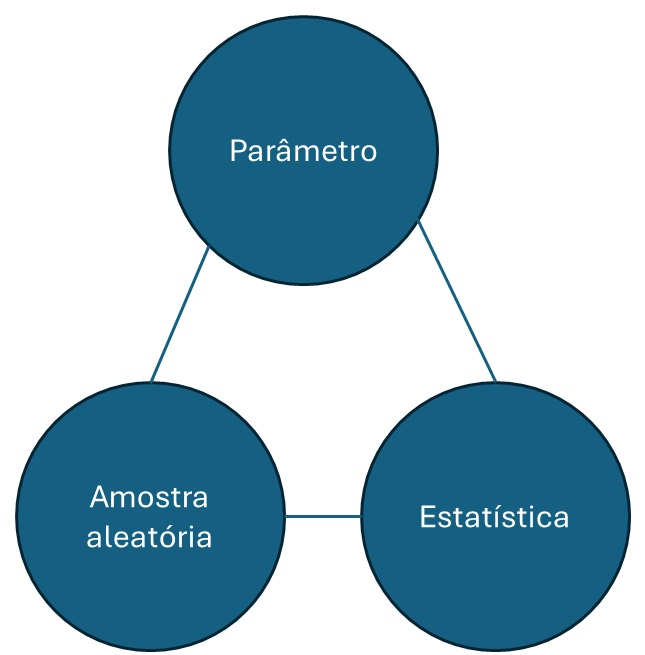
\includegraphics{fig_stat_geral.jpg}

}

\caption{A relação mais comum entre amostra, estatística e os parâmetros
populacionais}

\end{figure}%

Se a distribuição amostral da estatística não depende dos parâmetros,
dizemos que essa estatística é \textbf{ancilar}. A figura abaixo
representa a relação entre a amostra aleatória, os parâmetros e esse
tipo de estatística.

\begin{figure}

{\centering 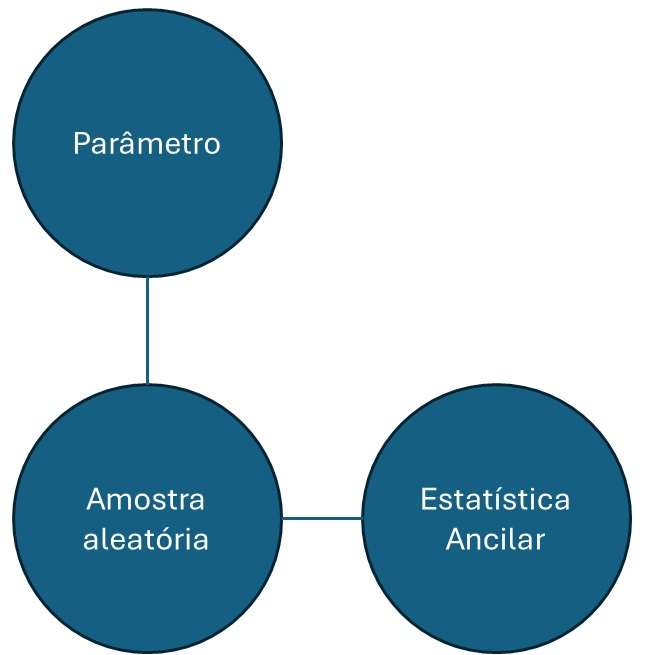
\includegraphics{fig_stat_ancilar.jpg}

}

\caption{Relação entre amostra, estatísticas ancilares e os parâmetros
populacionais}

\end{figure}%

\textbf{Exemplo} Seja \(X_1,\ldots,X_{n}\) uma amostra aleatória da
população Normal\((\mu,1)\). Sabemos que a distribuição amostral da
média amostral é
\[\bar{X}_n\sim\hbox{Normal}\left(\mu,\frac{1}{n}\right).\] Portanto,
\(\bar{X}_n\) carrega informação sobre \(\mu\). Considere agora a
estatística \[W=X_1-X_2.\] Note que \(W\) é uma combinação linear de
normais independentes, logo também possui distribuição normal. Como
\[E(W)=E(X_1)-E(X_2)=0\] e \[Var(W)=Var(X_1-X_2)=Var(X_1)+Var(X_2)=2,\]
temos que a distribuição amostral de \(W\) é Normal(0,2). Como essa
distribuição não depende de \(\mu\), temos que \(W\) não carrega
informação sobre o parâmetro e, portanto, é uma estatística ancilar.

Estatísticas ancilares possuem um papel relevante em problemas mais
complexos, mas que estão fora do escopo dessas notas de aula. Recomendo
ao leitor interessado a leitura de (Ghosh, Reid, and Fraser 2010),
disponível
\href{https://utstat.toronto.edu/reid/research/A20n41.pdf}{aqui}.

\section{Estatísticas suficientes}\label{estatuxedsticas-suficientes}

Uma estatística é dita ser suficiente para \(\theta\) se, quando
observada, ela permite descrever a distribuição da amostra aleatória sem
o conhecimento de \(\theta\). Segue a definição formal.

\textbf{Definição.} Uma estatística \(T\) é dita ser suficiente para
\(\theta\) se a distribuição \(X_1,\ldots,X_n|T=t\) não depende de
\(\theta\).

A figura abaixo mostra a relação entre a amostra aleatória, os
parâmetros e a estatística suficiente. Observe que a depenência da
amostra em relação aos parâmetros se dá através da estatítica
suficiente. 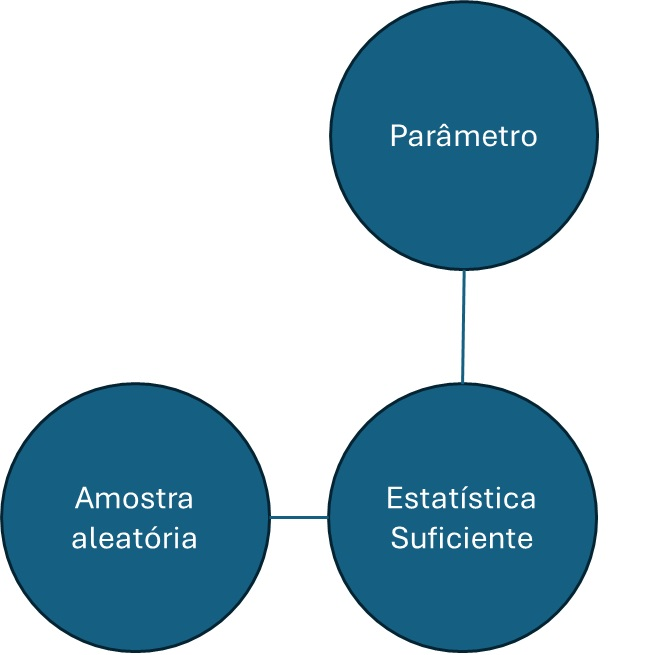
\includegraphics{fig_stat_suficiente.jpg}

Note que a própria amostra é uma estatística suficiente para \(\theta\).
De fato, considerando o caso discreto, pode-se notar que

\[P(\textbf{X}=\textbf{x}|\textbf{X}=\textbf{x},\boldsymbol{\theta})=\frac{P(\textbf{X}=\textbf{x},\textbf{X}=\textbf{x}|\boldsymbol{\theta})}{P(\textbf{X}=\textbf{x}|\boldsymbol{\theta})}=1,\]
que não depende de \(\theta\). O teorema a seguir é uma importante
ferramenta para encontrar estatísticas suficientes.

\textbf{Teorema do Critério da Fatoração de Neyman} Seja \(\textbf{X}\)
uma amostra aleatória cuja distribuição. Então, \(T\) é um estatística
suficiente para \(\theta\) se e somente se existem funções
\(h(\textbf{x})\) e \(g(T,\theta)\) tais que

\[\prod_{i=1}^nf(x_i|\theta)=h(\textbf{x})g(t,\theta)\] onde \(f\) é a
função de densidade ou a função de probabilidade da população.

\textbf{Exemplo} Seja \(X_1,\ldots,X_n\) uma amostra aleatória da
população Exponencial(\(\theta\)). Note que
\[\prod_{i=1}^n  f(x_i|\theta)=\prod_{i=1}^n \theta e^{-\theta x_i}=\underbrace{1}_{h(\textbf{x})}. \underbrace{\theta^ne^{-\theta\sum_{i=1}^n x_i}}_{g(\sum_{i=1}^n x_i,\theta)},\]
logo, pelo Teorema do Critério da Fatoração de Neyman,
\(T=\sum_{i=1}^{n}X_i\) é uma estatística suficiente para \(\theta\).

\textbf{Exemplo.} Seja \(X_1,\ldots,X_n\) uma amostra aleatória do
modelo \(X\sim\hbox{Poisson}(\lambda)\). Note que

\[P(\textbf{X}=\textbf{x}|\lambda)=\prod_{i=1}^n\frac{e^{-\lambda}\lambda^{x_i}}{x_i!}=\underbrace{\prod_{i=1}^n\frac{1}{x_i!}}_{h(\textbf{x})}.\underbrace{e^{-n\lambda}\lambda^{\sum_{i=1}^n x_i}}_{g(\sum_{i=1}^n x_i,\lambda)},\]
logo, pelo Teorema do Critério da Fatoração de Neyman,
\(T=\sum_{i=1}^n X_i\) é suficiente para \(\lambda\).

Quando há mais de uma estatística na fatoração, elas são denominadas
conjuntamente suficientes.

\textbf{Exemplo.} Seja \(X_1,\ldots,X_n\) uma amostra aleatória da
população \(\hbox{Normal}(\mu,\sigma^2)\). Note que
\[f(\textbf{x}|\mu,\sigma^2)=\prod_{i=1}^n\left(\frac{1}{2\pi\sigma^2}\right)^{1/2} e^{-\frac{1}{2\sigma^2}(x_i-\mu)^2}=\left(\frac{1}{2\pi\sigma^2}\right)^{n/2} e^{-\frac{1}{2\sigma^2}\sum_{i=1}^n(x_i-\mu)^2}.\]
Como
\[\sum_{i=1}^n(x_i-\mu)^2=\sum_{i=1}^n x_i^2 +n\mu^2-2\mu\sum_{i=1}^n x_i,\]
teremos que
\[f(\textbf{x}|\mu,\sigma^2)=\underbrace{1}_{h(\textbf{x})}.\underbrace{\left(\frac{1}{2\pi\sigma^2}\right)^{n/2} e^{-\frac{1}{2\sigma^2}\left(\sum_{i=1}^n x_i^2 +n\mu^2-2\mu\sum_{i=1}^n x_i\right)}}_{g( \sum_{i=1}^n x_{i},\sum_{i=1}^n x_i^2,\mu,\sigma^2)}.\]
Portanto, pelo Teorema do Critério da Fatoração de Neyman,
\(\sum_{i=1}^nX_i\) e \(\sum_{i=1}^n X_i^2\) são conjuntamente
suficientes para \(\mu\) e \(\sigma^2\).

Você deve ter notado que todas as distribuições acima pertencem à
família exponencial. O teorema abaixo generaliza a busca de estatísticas
suficientes dentro dessa família.

\textbf{Teorema} Se \(X_1,\ldots,X_n\) é uma amostra aleatória de uma
população na família exponencial, então
\[T=\left\{\sum_{i=1}^n T_1(X_i),\ldots,\sum_{i=1}^n T_k(X_i)\right\}\]
é uma estatística suficiente para \(\theta\).

\textbf{Exemplo} Seja \(X_1,\ldots,X_n\) uma amostra aleatória da
população Gama(\(\alpha\),\(\beta\)), cuja função densidade é dada por
\[f(x|\alpha,\beta)=\frac{\beta^\alpha}{\Gamma(\alpha)}x^{\alpha-1}e^{-\beta x},\]
com \(\alpha,\beta>0\). Notando que
\(x^\alpha=\exp\{\log(x^\alpha)\}=\exp\{\alpha\log(x)\}\), podemos
reescrever essa função densidade como

\[f(x|\alpha,\beta)=\underbrace{\frac{1}{x}}_{h(x)}.\underbrace{\frac{\beta^\alpha}{\Gamma(\alpha)}}_{a(\alpha,\beta)}\exp\left\{\underbrace{\alpha}_{w_1(\alpha,\beta)}\underbrace{\log(x)}_{t_1(x)}\underbrace{-\beta}_{w_2(\alpha,\beta)} \underbrace{x}_{t_2(x)}\right\}.\]
logo, a distribuição Gama pertence à família exponencial. Isso implica
que as estatísticas \(T_1=\sum_{i=1}^n \log(X_i)\) e
\(T_2=\sum_{i=1}^n X_i\) são conjuntamente suficientes para \(\alpha\) e
\(\beta\).

\textbf{Exemplo} Seja \(X_1,\ldots,X_n\) uma amostra aleatória da
população Beta(\(\alpha\),\(\beta\)), cuja função densidade é dada por
\[f(x|\alpha,\beta)=\frac{x^{\alpha-1}(1-x)^{\beta-1}}{B(\alpha,\beta)}.\]
onde \(x\in(0,1)\) e \(\alpha,\beta>0\). Notando que
\[x^\alpha=\exp\{\log(x^\alpha)\}=\exp\{\alpha\log(x)\},\] e
\[(1-x)^\beta=\exp\{\log((1-x)^\beta)\}=\exp\{\beta\log(1-x)\},\]

podemos reescrever essa função densidade como

\[f(x|\alpha,\beta)=\underbrace{\frac{1}{x(1-x)}}_{h(x)}.\underbrace{\frac{1}{B(\alpha,\beta)}}_{a(\alpha,\beta)}\exp\left\{\underbrace{\alpha}_{w_1(\alpha,\beta)}\underbrace{\log(x)}_{t_1(x)}+\underbrace{\beta}_{w_2(\alpha,\beta)} \underbrace{\log(1-x)}_{t_2(x)}\right\}.\]
logo, a distribuição Beta pertence à família exponencial. Isso implica
que as estatísticas \(T_1=\sum_{i=1}^n \log(X_i)\) e
\(T_2=\sum_{i=1}^n \log(1-X_i)\) são conjuntamente suficientes para
\(\alpha\) e \(\beta\).

Vejamos alguns exemplos fora da família exponencial.

\textbf{Exemplo.} Seja \(X_1,\ldots,X_n\) uma amostra aleatória da
população Uniforme(0,\(\theta\)). Note que

\[\prod_{i=1}^n f(x_i|\theta)=\prod_{i=1}^n \frac{1}{\theta}I(x_i\leq \theta)=\frac{1}{\theta^n}\prod_{i=1}^{n}I(x_i\leq \theta).\]
O produtório acima é igual a 1 se e somente se todas as observações
forem menores ou iguais que \(\theta\). Para que isto ocorra, basta que
a maior das observações seja menor que \(\theta\). Denotando a
estatística máximo amostral por \(X_{(n)}\), teremos

\[\prod_{i=1}^nf(x_i|\theta)=\underbrace{1}_{h(\textbf{x})}.\underbrace{\frac{1}{\theta^n}I(x_{(n)}\leq\theta)}_{g(x_{(n)},\theta)},\]
logo, pelo Teorema do Critério da Fatoração de Neyman, teremos que
\(T=X_{(n)}\) é suficiente para \(\theta\).

\textbf{Importante} Sejam \(x_{(1)}\) e \(x_{(n)}\) as estatísticas
mínimo e máximo de uma amostra de tamanho \(n\). Então: -
\(\prod_{i=1}^n I(x_i\leq \theta)=I(x_{(n)}\leq \theta)\) -
\(\prod_{i=1}^n I(x_i\geq \theta)=I(x_{(1)}\geq \theta)\) -
\(\prod_{i=1}^n I(\alpha\leq x_i\leq \beta)=I(\alpha\leq x_{(1)})I(x_{(n)}\leq \beta)\)

\textbf{Exemplo.} Seja \(X_1,\ldots,X_n\) uma amostra aleatória da
população cuja função densidade é dada por

\[f(x|\mu)=e^{-(x-\mu)}I(x\geq \mu),\] onde \(\mu>0\). Esse modelo é
conhecido como exponencial deslocada. Contudo, como os valores de \(x\)
dependem de \(\mu\), esta distribuição não está na família exponencial.
Observe que
\[\prod_{i=1}^n f(x_i|\mu)=\prod_{i=1}^n e^{-(x_i-\mu)}I(x_i\geq \mu)=e^{-\sum_{i=1}^n x_i}e^{n\mu}\prod_{i=1}^{n}I(x_i\geq \mu).\]
O produtório acima é igual a 1 se e somente se todas as observações
forem maiores ou iguais que \(\mu\). Para que isto ocorra, basta que
\(x_{(1)}\) seja maior que \(\mu\). Então, teremos que

\[\prod_{i=1}^nf(x_i|\theta)=\underbrace{e^{-\sum_{i=1}^n x_i}}_{h(\textbf{x})}.\underbrace{e^{n\mu}I(x_{(1)}\geq \mu)}_{g(x_{(1)},\mu)},\]
logo, pelo Teorema do Critério da Fatoração de Neyman, teremos que
\(T=X_{(1)}\) é suficiente para \(\mu\).

\textbf{Exemplo.} Seja \(X_1,\ldots,X_n\) uma amostra aleatória da
população Uniforme(\(\alpha,\beta\)), cuja densidade é dada por

\[f(x|\alpha,\beta)=\frac{1}{\beta-\alpha}I(\alpha\leq x\leq \beta),\]
onde \(\alpha<\beta\). Sem perda de generalidade, podemos reescrever
\[I(\alpha\leq x\leq \beta)=I(\alpha\leq x)I(x\leq\beta),\] logo,

\[\begin{align}\prod_{i=1}^n f(x_i|\alpha,\beta)&=\prod_{i=1}^n \frac{1}{\beta-\alpha}I(\alpha\leq x_i)I(x_i\leq\beta)\\&=\underbrace{1}_{h(\textbf{x})}.\underbrace{\frac{1}{(\beta-\alpha)^n}I(\alpha\leq x_{(1)})I(x_{(n)}\leq\beta)}_{g(x_{(1)},x_{(n)},\alpha,\beta
)}.\end{align}\] logo, pelo Teorema do Critério da Fatoração de Neyman,
teremos que \(X_{(1)}\) e \(X_{(n)}\) são conjuntamente suficientes para
\(\alpha\) e \(\beta\).

Em determinado momento do curso, vamos estar interessados em
estatísticas baseadas em estatísticas suficientes. Segue um importante
resultado.

\textbf{Proposição.} Seja \(T\) uma estatística suficiente. Defina outra
estatística \(W=g(T)\). Se \(g(.)\) possui inversa, então \(W\) também é
suficiente.

\textbf{Nota.} Para mostrar que existe uma função inversa entre \(A\) e
\(B\) você deve mostrar que é possível escrever \(A\) como função de
\(B\) ou seja \[A=f(B)\] e depois deve mostrar que é possível escrever
\(B\) como função de \(A\), ou seja \[B=h(A).\] Desse modo a função
inversa de \(f(.)\) é \(h(.)\) ( e vice e versa).

\textbf{Exemplo.} Para uma amostra aleatória proveniente de um população
Poisson(\(\lambda\)), mostramos que \(T=\sum_{i=1}^n X_i\) é suficiente
para \(\lambda\). Observe que
\[\bar{X}_n=\frac{1}{n}\sum_{i=1}^n X_i=\frac{T}{n},\] ou seja,
\(\bar{X}_n\) pode ser escrita como função da estatística suficiente
\(T\). Além disso, é imediato que \(T=n\bar{X}_n\). Portanto, \(T\) pode
ser escrito como função de \(\bar{X}_n\), o que implica que
\(\bar{X}_n\) também é suficiente para \(\lambda\).

\subsection{Estatística suficiente e
completa}\label{estatuxedstica-suficiente-e-completa}

Seja \(T\) uma estatística suficiente e \(U\) uma ancilar. Existem
situações nas quais as estatísticas não são independentes, conforme
vemos na figura abaixo. Quando isso ocorre, pode ser vantajoso utilizar
o par \((T,U)\) para realizar inferências (\(U\) é denominado
complemento ancilar para \(T\)).

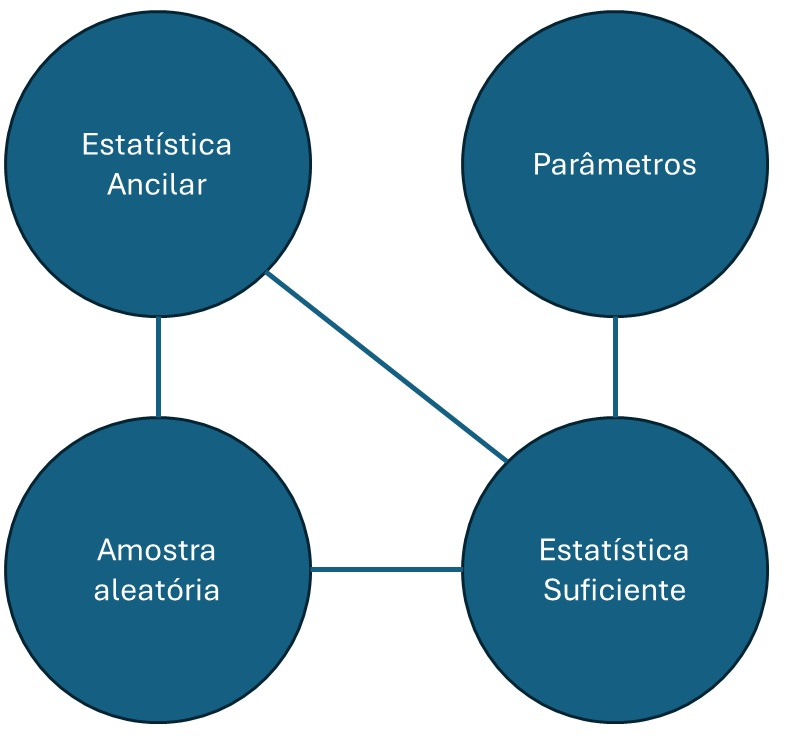
\includegraphics{fig_stat_suficiente_ancilar.jpg} Uma classe de
estatísticas suficientes que não necessitam de complementos ancilares é
definida abaixo.

\textbf{Definição (Estatística suficiente e completa).} Seja \(T\) uma
estatística suficiente. Dizemos que ela é completa se, para qualquer
função real \(g(.)\), tem-se que, se \(E(g(T)|\theta)=0\) para todo
\(\theta\), então \(g(t)=0\) para todo \(t\).

\textbf{Teorema de Basu.} Estatísticas suficientes e completas são
independentes de estatísticas ancilares.

Portanto, na existência de estatísticas suficientes e completas, estas
são as únicas necessárias para realizar inferências sobre os parâmetros
populacionais (não há necessidade de se procurar por algum complemento
ancilar). A figura abaixo ilustra as relações entre a amostra aleatória,
os parâmetros e as estatísticas ancilares e completas.

\begin{figure}

{\centering 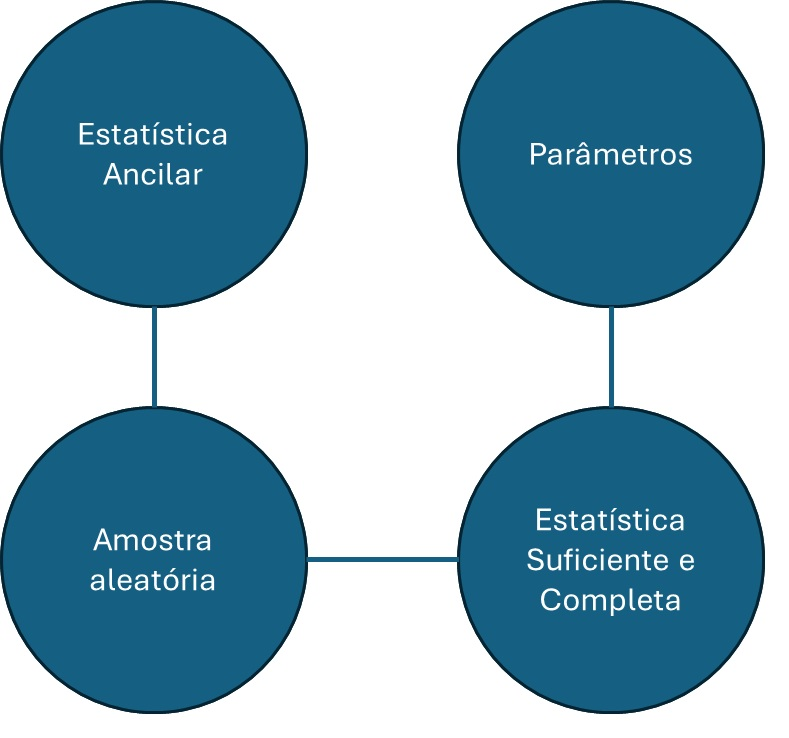
\includegraphics{fig_stat_completa_ancilar.jpg}

}

\caption{Estatísticas suficientes e completas carregam toda a informação
necessária para realizar inferências sobre os parâmetros.}

\end{figure}%

Veremos abaixo algumas situações nas quais podemos encontrar
estatísticas suficientes e completas.

\textbf{Teorema} Suponha que \(X_1,\ldots,X_n\) é uma amostra aleatória
de uma população pertencente à família exponencial. Então,
\(T(\textbf{X})=(\sum_{i=1}^nT_1(X_i),\ldots,\sum_{i=1}^nT_k(X_i))\) é
uma estatística suficiente e completa se a imagem de
\((w_1(\theta),\ldots,w_k(\theta))\) contém um retângulo aberto em
\(\mathbb{R}^k\)

\textbf{Nota.} No teorema acima, se \(k=1\), basta que a imagem de
\(w(\theta)\) contenha um intervalo aberto na reta. Se \(k=2\), basta
que a imagem de \((w_1(\theta),w_2(\theta))\) contenha um retângulo
aberto em \(\mathbb{R}^2\), e assim por diante.

\textbf{Exemplo.} Seja \(X\) uma variável aleatória com distribuição
Poisson(\(\lambda\)). Recordemos que essa distribuição pertence à
família exponencial, pois

\[P(X=x|\lambda)=\underbrace{\frac{1}{x!}}_{h(x)}\underbrace{e^{-\lambda}}_{a(\lambda)}\exp\{\;\underbrace{x}_{t(x)}.\underbrace{\log(\lambda)}_{w(\lambda)}\;\}.\]
Portanto, a estatística \(T=\sum_{i=1}^nX_i\) é suficiente. Note que a
imagem que \(\log(\lambda)\) é \(\mathbb{R}\), que contém infinitos
intervalos abertos. Portanto, a estatística \(T\) também é completa.

O teorema abaixo mostra a existência de uma estatística suficiente e
completa em outra família de distribuições.

\textbf{Teorema.} Suponha que
\[f(x|\beta)=\frac{h(x)}{H(\beta)-H(0)}I(0<x\leq \theta),\] onde
\(h(x)\geq 0\) e \[H(x)=\int_0^x h(y)dy.\]

Então, considerando uma amostra aleatória desse modelo, a estatística
\(X_{(n)}\) é suficiente e completa para \(\beta\). Alternativamente,
seja \[f(x|\alpha)=\frac{h(x)}{1-H(\alpha)}I(x\geq \alpha),\] onde
\(h(x)\leq 0\), \(H(x)=\int_{0}^xh(y)dy\) e
\(\lim_{x\rightarrow \infty}H(x)=1\). Então \(X_{(1)}\) é uma
estatística suficiente e completa para \(\alpha\).

\textbf{Exempo.} Considere o modelo Uniforme\((0,\theta)\), cuja função
densidade é dada por \[f(x|\theta)=\frac{1}{\theta}I(0<x\leq \theta).\]
Vamos verificar se essa distribuição pode ser escrita conforme o
descrito no teorema acima. Podemos identificar \(h(x)=1\). Logo,
\[H(x)=\int_0^x 1dy=\left. y\right|_{0}^x=x.\] Como \(H(\theta)=\theta\)
e \(H(0)=0\), teremos que
\[f(x|\theta)=\frac{1}{\theta}I(0<x\leq\theta)=\frac{h(x)}{H(\theta)-H(0)}I(0<x\leq\theta)\]
e \(X_{(n)}\) é uma estatística suficiente e completa para \(\theta\).

\textbf{Exempo.} Considere o modelo exponencial deslocada, cuja função
densidade é dada por
\[f(x|\mu)=e^{-(x-\mu)}I(x\geq \mu)=\frac{e^{-x}}{e^{-\mu}}I(x\geq \mu),.\]
onde \(\mu>0\). Vamos verificar se essa distribuição pode ser escrita
conforme o descrito no teorema acima. Podemos identificar
\(h(x)=e^{-x}\). Logo,
\[H(x)=\int_{0}^x  e^{-y}dy=\left. -e^{-y}\right|_0^x=-e^{-x}+1.\] Como
\(H(\mu)=1-e^{-\mu}\) e \[\lim_{x\rightarrow\infty }H(x)=1\], teremos
que
\[f(x|\theta)=e^{-(x-\mu)}I(x\geq\mu)=\frac{e^{-x}}{1-(1-e^{-\mu})}I(x\geq\mu)=\frac{h(x)}{1-H(x)}I(x\geq\mu)\]
e \(X_{(1)}\) é uma estatística suficiente e completa para \(\mu\).

\bookmarksetup{startatroot}

\chapter{Estimação pontual}\label{estimauxe7uxe3o-pontual}

\section{Estimador, estimativa, erro quadrático médio e
consistência}\label{estimador-estimativa-erro-quadruxe1tico-muxe9dio-e-consistuxeancia}

A palavra estimar possui vários significados na língua portuguesa. Em um
de seus verbetes, estimar significa apreciação ou avaliação. Neste
sentido, a estimação pontual refere-se a um conjunto de técnicas para
encontrar uma estatística para avaliar alguma característica da
população.

\textbf{Definição} Estimador é uma estatística criada com o objetivo de
estimar os parâmetros populacionais. Seu valor observado é denominado
estimativa.

Por ser uma estatística, o estimador possui uma distribuição amostral.
Considerando seu objetivo primário de estimar \(\theta\), é natural que
o estimador produza estimativas próximas deste valor.

Seja \(T\) um estimador para \(\theta\). Definimos o erro quadrático
médio por

\[EQM_T(\theta)=E(T-\theta)^2.\] Quanto menor for o erro quadrático
médio, maior é a capacidade do estimador produzir, em média, estimativas
próximas de \(\theta\). Pode-se notar que

\[\begin{align}EQM_T(\theta)&=E\left(T-E(T)+E(T)-\theta\right)^2\\&=E\left( (T-E(T))^2+(E(T)-\theta)^2- (T-E(T))(E(T)-\theta)\right)\\&=Var(T)+(E(T)-\theta)^2\\&=SE(T)^2+\hbox{Vício}_T(\theta)^2.\end{align}\]
onde \[\hbox{Vício}_T(\theta)=E(T)-\theta\] e \[SE(T)=\sqrt{Var(T)}.\]

Vamos analisar as parcelas dessa decomposição em separado. O termo
\(E(T)-\theta\) é denominado vício (do estimador). - Se o vício é nulo,
o estimador é dito ser não viciado. - Se o vício é positivo, o estimador
tende a superestimar \(\theta\). - Se o vício é negativo, o estimador
tende a subestimar \(\theta\). O termo \(SE(T)\) é denominado erro
padrão (\emph{standard error}) e é uma medida de acurácia do estimador.

\textbf{Nota.} O erro quadrático médio é utilizado para comparar
estimadores. Já o erro padrão é uma importante medida que precisa ser
reportada junto com a estimativa pontual.

\textbf{Exemplo.} Seja \(X_1,\ldots,X_n\) uma amostra aleatória de um
membro da família de distribuições com variância finita. Sejam
\(E(X)=\mu\) e \(\sigma^2=Var(X)\). Considere o estimador \(\bar{X}_n\)
para \(\mu\). Como a família não é paramétrica, não sabemos a
distribuição amostral de \(\bar{X}_n\). Contudo, tem-se que
\[E(\bar{X}_n)=E\left(\frac{1}{n}\sum_{i=1}^n X_i\right)=\frac{1}{n}\sum_{i=1}^nE(X_i)=E(X)=\mu\]
logo, o estimador \(\bar{X}_n\) é não viciado para \(\mu\). Além disso,
\[Var(\bar{X}_n)=Var\left(\frac{1}{n}\sum_{i=1}^{n}X_i\right)=\frac{1}{n^2}\sum_{i=1}^n Var(X_i)=\frac{\sigma^2}{n}\]
logo, o erro quadrático de \(\bar{X}\) é
\[EQM_{\bar{X}_n}(\mu)=\frac{\sigma^2}{n}.\] Observe que esse erro
quadrático médio é inversamente proporcional ao tamanho da amostra.
Portanto, quanto maior o tamanho da amostra, mais próximas de \(\mu\)
estarão as estimativas produzidas por \(\bar{X}_n\).

O erro padrão é dado por \[SE(\bar{X}_n)=\frac{\sigma}{\sqrt{n}},\] mas
só pode ser reportado se \(\sigma\) for conhecido. É possível mostrar
que, sob as mesmas condições, o estimador
\[S^2=\frac{1}{n-1}\sum_{i=1}^n (X_i-\bar{X}_n)^2\] é não viciado para
\(\sigma^2\).

No exemplo acima, vimos que o erro quadrático médio de \(\bar{X}_n\)
tende a zero na medida que aumentamos o tamanho da amostra. Estimadores
com essa característica são denominados consistentes.

Uma sequência \(T_n=T_n(X_1,\ldots,X_n)\) de estimadores para \(\theta\)
é consistente se, para qualquer \(\varepsilon>0\) e \(\theta\in\Theta\),
\[\lim_{n\rightarrow\infty} P(|T_n-\theta|<\varepsilon)=1.\]

Intuitivamente, quanto maior é o tamanho da amostra, maior é a
probabilidade do estimador estar arbitrariamente próximo de \(\theta\).
O resultado abaixo relaciona a consistência com o erro quadrático médio.

\textbf{Proposição.} Seja \(T_n=T(X_1,\ldots,X_n)\) uma sequência de
estimadores. Se, para todo \(\theta\),
\[\lim_{n\rightarrow\infty}EQM_{T_n}(\theta)=0,\] então \(T_n\) é
consistente.

\textbf{Exemplo}. Considere uma amostra aleatória de uma população com
variância finita. Mostramos anteriormente que
\[EQM_{\bar{X}_n}(\mu)=\frac{\sigma}{n}.\] Como
\[\lim_{n\rightarrow\infty}\frac{\sigma}{n}=0,\] temos que \(\bar{X}_n\)
é um estimador consistente.

\section{O princípio da
substituição}\label{o-princuxedpio-da-substituiuxe7uxe3o}

Discutimos anteriormente que as características de interesse presentes
na população são funções dos parâmetros populacionais. Ao se obter uma
estimativa para \(\theta\), é natural que essa estimativa seja
utilizadas para estimar qualquer função de \(\theta\).

\textbf{Princípio da substituição.} Seja \(T\) uma estimador para
\(\theta\). Então, para qualquer função real \(g(.)\), \(g(T)\) será um
estimador para \(g(\theta)\).

\textbf{Exemplo} Considere novamente uma amostra aleatória de um membro
da família de distribuições com variância finita. Vimos que \(S^2_n\) é
um estimador não viciado para \(Var(X)=\sigma^2\). Então, pelo princípio
da substituição, \[S_n=\sqrt{S^2_n}\] é um estimador para \(\sigma\).
Também vimos que \(\bar{X}_n\) é um estimador para \(\mu=E(X)\) e que
seu erro padrão é \[SE(\bar{X}_n)=\frac{\sigma}{\sqrt{n}}.\] Logo, um
estimador para erro padrão de \(\bar{X}_n\) é

\[\widehat{SE}(\bar{X}_n)(\mu)=\frac{S_n}{\sqrt{n}}.\]

\textbf{Exemplo.} Foram coletados o peso em gramas de 100 bebês
recém-nascidos no estado do Amazonas em 2010. A estimativa obtida para a
média foi \(\bar{x}=3.226,85 g\). O desvio padrão amostral foi 474,556.
Logo, o erro padrão estimado para a média foi

\[\hat{SE}(\bar{X}_n)=\frac{474,556g}{\sqrt{100}}=47,4556g.\] Portanto,
a estimativa possui um erro de 47,4556\(g\). É usual escrever
\(3.226,85g\pm47,4556g\).

Isso implica que há evidências de que nossa estimativa está correta na
casa das unidades de milhar, mas pode conter erros nas casas anteriores.
A estratégia para diminuir o erro padrão é aumentar o tamanho da
amostra.

Seja \(T\) um estimador para \(\theta\) e considere novamente o problema
de estimar \(g(\theta)\). O valor da função \(g(.)\) quando \(t\) está
na vizinhança de \(\theta\) pode ser aproximado por
\[g(t)\approx g(\theta)+(t-\theta)g'(\theta),\] onde \(g'\) é derivada
de \(g\). Observe que \[g(t)-g(\theta)\approx (t-\theta)g'(\theta),\]
logo
\[\underbrace{E\left(g(T_n)-g(\theta)\right)^2}_{EQM_{g(T_n)}(g(\theta))}\approx \underbrace{E\left(T-\theta\right)^2}_{EQM_{T_n}(\theta)} [g'(\theta)]^2\]

Portanto, se \(T_n\) for consistente, então \(g(T_n)\) também será
consistente. Além disso, pode-se mostrar que\\
\[\underbrace{E(g(T_n))-g(\theta)}_{\hbox{Vício}_{g(T_n)}(g(\theta))}\approx \underbrace{(E(T_n )-\theta)}_{\hbox{Vício}_{T_n}(\theta)}g'(\theta),\]
e, se \(T_n\) é não viciado, teremos que \(g(T_n)\) será aproximadamente
não viciado. Além disso,

\[Var(g(T_n))\approx \underbrace{E(T_n-\theta)^2}_{EQM_{T_n}(\theta)}g'(\theta)^2.\]
e, se \(T_n\) é não viciado, o erro padrão de \(g(T_n)\) é aproximado
por \[SE(g(T_n))\approx SE(T_n)|g'(\theta)|.\]

\textbf{Importante.} A aproximação
\[g(t)-g(\theta)\approx (t-\theta)g'(\theta)\] é razoável apenas quando
\(t\) está na vizinhança de \(\theta\). Para que os resultados
utilizando esperança e variância sejam razoáveis, é necessário que a
distribuição amostral de \(T_n\) esteja bem concentrada em torno de
\(\theta\), o que é obtido na prática com um tamanho grande de amostra,
desde que \(T_n\) seja consistente.

\section{Método dos momentos}\label{muxe9todo-dos-momentos}

O \(k\)-ésimo momento da população é definido por \(\mu_k=E(X^k)\).
Defina o \(k\)-ésimo momento amostral por
\[\hat{\mu}_k=\frac{1}{n}\sum_{i=1}^n X_i^k\] Observe que, ao fazer
\(X_i^k=Y_i\), teremos que \(\hat{\mu}_k=\bar{Y}_n\). Isso nos permite
provar que:

\begin{itemize}
\tightlist
\item
  \(\hat{\mu}_k\) é um estimador não viciado para \(\mu_k\)
\item
  \(SE(\hat{\mu})=\sqrt{Var(X^k)/n}\)
\item
  \(EQM_{\hat{\mu}_k}(\mu_k)=Var(X^k)/n\)
\item
  \(\hat{\mu}_k\) é consistente
\end{itemize}

Além disso, para \(n\) suficientemente grande, pelo Teorema Central do
Limite
\[\hat{\mu}_k\approx \hbox{Normal}\left(\mu_k,\frac{Var(X^k)}{n}\right)\]

\textbf{Exemplo} Seja \(X_1,\ldots,X_n\) uma amostra aleatória da
população Poisson(\(\lambda\)). Sabemos que o primeiro momento
populacional é \(E(X)=\lambda\). Logo, a média amostral é um estimador
não viciado e consistente para \(\lambda\). Além disso, como
\[Var(X)=\lambda,\] para \(n\) suficientemente grande,

\[\bar{X}\approx \hbox{Normal}\left(\lambda,\frac{\lambda}{n}\right).\]
Note que é possível trabalhar com a distribuição exata de \(\bar{X}_n\),
uma vez que \[\sum_{i=1}^n X_i\sim\hbox{Poisson}(n\lambda)\] e
\[P(\bar{X}_n=\bar{x}|\lambda)=P\left(\left.\sum_{i=1}^n X_i=n\bar{x}\right|\lambda\right).\]

Considere uma amostra aleatória de uma população com parâmetros
\(\theta_1,\ldots,\theta_k\). Suponha que os \(k\) primeiros momentos
podem ser escritos como função dos parâmetros, ou seja, existem funções
\(g_j(.)\), \(j=1,\ldots,k\) tais que
\[\mu_k=g_j(\theta_1,\ldots,\theta_k).\] Suponha ainda que existem
funções \(h_j(.)\), \(j=1,\ldots,k\), tais que
\[\theta_j=h_j(\mu_1,\ldots,\mu_k).\] O método dos momentos consiste em
encontrar os estimadores \(\hat{\theta}_1,\ldots,\hat{\theta}_k\)
computando \[\hat{\theta}_j=h_j(\hat{\mu}_1,\ldots,\hat{\mu}_k).\]

Em outras palavras, o método dos momentos consiste em utilizar os
momentos amostrais e aplicar o princípio da substituição para obter
estimativas dos parâmetros. Como os momentos amostrais são não viciados
e consistentes, podemos obter as seguintes propriedades:

\begin{enumerate}
\def\labelenumi{\arabic{enumi}.}
\tightlist
\item
  \(\hat{\theta}_j\) é aproximadamente não viciado
\item
  \(\hat{\theta}_j\) é consistente
\end{enumerate}

Além disso, a distribuição amostral dos estimadores de momentos é
aproximadamente normal. Quando há apenas um parâmetro, essa aproximação
é dada por

\[\hat{\theta}\approx \hbox{Normal}\left( \theta_j,\frac{Var(X)}{n}\left[\frac{d}{d\mu}h(\mu)\right]^2 \right).\]

\textbf{Exemplo} Seja \(X_1,\ldots,X_n\) uma amostra aleatória da
população Exponencial(\(\theta\)). O primeiro momento amostral é
\[\mu=E(X)=\frac{1}{\theta}=g(\theta).\] Podemos então escrever
\(\theta\) como função do primeiro momento amostral:
\[\theta=\frac{1}{\mu}=h(\mu)\] Logo, o estimador obtido via método dos
momentos para \(\theta\) é
\[\hat{\theta}=\frac{1}{\hat{\mu}}=\frac{1}{\bar{X}_n}.\] Como
\[Var(X)=\frac{1}{\theta^2}\] e
\[\frac{d}{d\mu}h(\mu)=-\frac{1}{\mu}^2=\left(\frac{1}{\mu}\right)^2=\theta^2,\]
teremos que, para \(n\) suficientemente grande, sua distribuição
amostral será
\[\hat{\theta}\approx N\left(\theta,\frac{Var(X)}{n}h'(\mu)^2\right)=N\left(\theta,\frac{\theta^2}{n}\right)\]

\textbf{Exemplo} Seja \(X_1,\ldots,X_n\) uma amostra aleatória da
população Geométrica(\(\theta\)). O primeiro momento amostral é
\[\mu=E(X)=\frac{1-\theta}{\theta}=g(\theta).\] Podemos então escrever
\(\theta\) como função do primeiro momento amostral:
\[\theta=\frac{1}{1+\mu}=h(\mu)\] Logo, o estimador obtido via método
dos momentos para \(\theta\) é
\[\hat{\theta}=\frac{1}{1+\hat{\mu}}=\frac{1}{1+\bar{X}_n}.\] Como
\[Var(X)=\frac{1-\theta}{\theta^2},\] e
\[\frac{d}{d\mu}h(\mu)=-\frac{1}{(1+\mu)^2}=\left(\frac{1}{1+\mu}\right)^2=\theta^2,\]
teremos que, para \(n\) suficientemente grande, sua distribuição
amostral será
\[\hat{\theta}\approx N\left(\theta,\frac{Var(X)}{n}h'(\mu)^2\right)=N\left(\theta,\frac{\theta^2(1-\theta)}{n}\right)\]

É possível encontrar a distribuição exata de \(\hat{\theta}\). Para
tanto, lembremos que
\[\sum_{i=1}^n X_i\sim \hbox{Binomial Negativa}(n,\theta),\] logo,
\[\begin{align}P\left(\hat{\theta}=c|\theta\right)&=P\left(\left.\frac{1}{1+\bar{X}_n}=c\right|\theta\right)=P\left(\left.\bar{X}_n=\frac{1}{c}-1\right|\theta\right)\\&=
P\left(\left.\sum_{i=1}^n X_i=n\left(\frac{1}{c}-1\right)\right|\theta\right).
\end{align}\]

\textbf{Exemplo.} Seja \(X_1,\ldots,X_n\) uma amostra aleatória da
distribuição Gama(\(\alpha,\beta\)). A esperança e a variância desse
modelo são \[E(X)=\frac{\alpha}{\beta}\] e
\[Var(X)=\frac{\alpha}{\beta^2}.\] Como \(E(X^2)=Var(X)+E(X)^2\),
podemos deduzir que \[E(X^2)=\frac{\alpha^2+\alpha}{\beta^2}.\] Então,
os dois primeiros momentos escritos como função de \(\alpha\) e
\(\beta\) são
\[\begin{align}\mu_1&=\frac{\alpha}{\beta^2}=g_1(\alpha,\beta),\\
\mu_2&=\frac{\alpha^2+\alpha}{\beta^2}=g_2(\alpha,\beta).\end{align}\]
Podemos então escrever \(\alpha\) e \(\beta\) como função de \(\mu_1\) e
\(\mu_2\):
\[\begin{align}\alpha&=\frac{\mu_1^2}{\mu_2-\mu_1^2}=\frac{\mu_1^2}{Var(X)}=h_1(\mu_1,\mu_2),\\
\beta&=\frac{\mu_1}{\mu_2-\mu_1^2}=\frac{\mu_1}{Var(X)}=h_2(\mu_1,\mu_2).\end{align}\]
Portanto os estimadores para \(\alpha\) e \(\beta\) obtidos via método
dos momentos são:
\[\begin{align}\hat{\alpha}&=\frac{\bar{X}_n^2}{S^2_n}=h_1(\mu_1,\mu_2),\\
\hat{\beta}&=\frac{\bar{X}_n}{S^2_n}=h_2(\mu_1,\mu_2).\end{align}.\]

\textbf{Exemplo.} Seja \(X_1,\ldots,X_n\) uma amostra aleatória da
distribuição Beta(\(\alpha,\beta\)). A esperança e a variância desse
modelo são \[E(X)=\frac{\alpha}{\alpha+\beta}\] e
\[Var(X)=\frac{\alpha\beta}{(\alpha+\beta)^2(\alpha+\beta+1)}.\] Como
\(E(X^2)=Var(X)+E(X)^2\), podemos deduzir que
\[E(X^2)=\frac{\alpha^2}{(\alpha+\beta)^2}+\frac{\alpha\beta}{(\alpha+\beta)^2(\alpha+\beta+1)}.\]
Então, os dois primeiros momentos escritos como função de \(\alpha\) e
\(\beta\) são
\[\begin{align}\mu_1&=\frac{\alpha}{\alpha+\beta}=g_1(\alpha,\beta),\\
\mu_2&=\frac{\alpha^2}{(\alpha+\beta)^2}+\frac{\alpha\beta}{(\alpha+\beta)^2(\alpha+\beta+1)}=g_2(\alpha,\beta).\end{align}\]
Podemos então escrever \(\alpha\) e \(\beta\) como função de \(\mu_1\) e
\(\mu_2\):
\[\begin{align}\alpha&=\frac{\mu_1^2-\mu_1\mu_2}{\mu_2-\mu_1^2}=\mu_1\left(\frac{\mu_1(1-\mu_1)}{Var(X)}-1\right)=h_1(\mu_1,\mu_2),\\
\beta&=(1-\mu_1)\left(\frac{\mu_1(1-\mu_1)}{Var(X)}-1\right)=h_2(\mu_1,\mu_2).\end{align}\]
Portanto os estimadores para \(\alpha\) e \(\beta\) obtidos via método
dos momentos são:
\[\begin{align}\hat{\alpha}&=\bar{X}_n\left(\frac{\bar{X}_n(1-\bar{X}_n)}{S_n^2}-1\right),\\
\hat{\beta}&=(1-\bar{X}_n)\left(\frac{\bar{X}_n(1-\bar{X}_n)}{S_n^2}-1\right).\end{align}\]

Para o caso de \(q\) parâmetros, é possível mostrar que a distribuição
aproximada dos estimadores de momentos é

\[\hat{\theta}_j\approx \hbox{Normal}\left(\theta_j,\frac{1}{n}\sum_{r=1}^k\sum_{s=1}^k\sigma_{r,s}\frac{\partial}{\partial\mu_r}h_j\frac{\partial}{\partial\mu_s}h_j\right),\]
onde \[\sigma_{r,s}=Cov(X^r,X^s).\]

\section{A função de distribuição empírica e o método
bootstrap}\label{a-funuxe7uxe3o-de-distribuiuxe7uxe3o-empuxedrica-e-o-muxe9todo-bootstrap}

\bookmarksetup{startatroot}

\chapter*{References}\label{references}
\addcontentsline{toc}{chapter}{References}

\markboth{References}{References}

\phantomsection\label{refs}
\begin{CSLReferences}{1}{0}
\bibitem[\citeproctext]{ref-ghosh2010ancillary}
Ghosh, Malay, N Reid, and DAS Fraser. 2010. {``Ancillary Statistics: A
Review.''} \emph{Statistica Sinica}, 1309--32.

\end{CSLReferences}



\end{document}
